\section{Введение}

\begin{frame}
    \frametitle{Течение через пористую среду}

    \begin{columns}
    \begin{column}{0.6\textwidth}
        \begin{figure}[H]
            \centering
            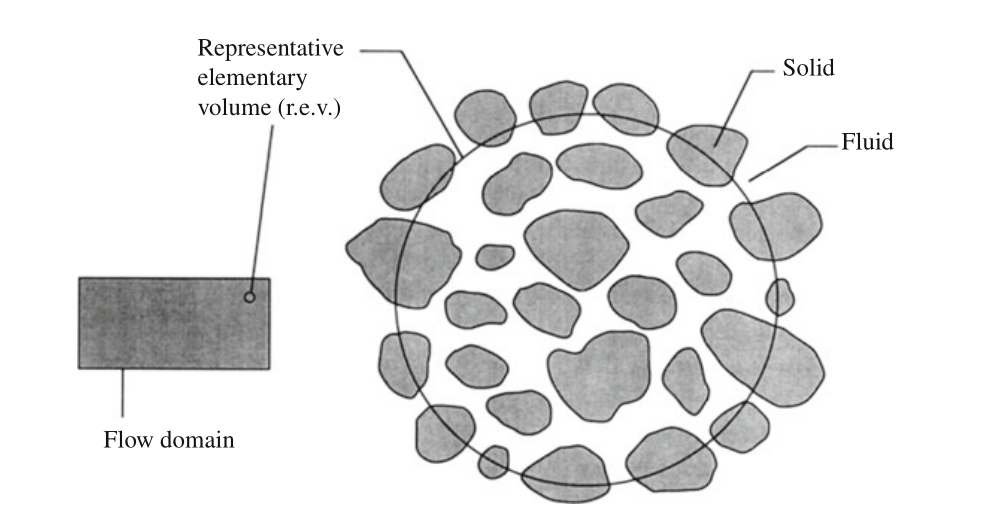
\includegraphics[width=\textwidth]
            {img/porous-medium.png}
        \end{figure}
    \end{column}
    \begin{column}{0.4\textwidth}
            Макроскопические уравнения течения получаются
            усреднением обычных уравнений по объёмам,
            содерживающим много пор.
    \end{column}
    \end{columns}

\end{frame}

\begin{frame}
    \frametitle{Скорость фильтрации и уравнения непрерывности}
    Скорость фильтрации - средняя скорость жидкости в свободном
    пространстве внутри пор.
    \[
    \vec v = \varphi \vec V_f
    \] 
    где \(\varphi\) - пористость среды, 
    \(\vec V_f\) - средняя скорость течения через объем, не
    содержащий поров.

    \begin{block}{Уравнеие непрерывности для каждого компонента}
        \begin{equation}
            \varphi \frac{\partial \rho_i}{\partial t}
            + div (\rho_i \bm{v}_i) = 0
        \end{equation}
    \end{block}
\end{frame}

\begin{frame}
    \frametitle{Закон Дарси: проницаемость}
    \begin{columns}
    \begin{column}{0.6\textwidth}
        \begin{block}{Закон Дарси для каждого компонента}
            \begin{equation}
                \mathbf{v}_i = -\frac{1}{\mu_i} K \cdot f_i (s)
                \cdot \nabla P
            \end{equation}
        \end{block}
        \(K\) --- коэффициент проницаемости,

        \(f\) --- относительная фазовая проницаемость,

        \(\mu\) --- динамическая вязкость,

        \(s\) --- газонасыщенность.
    \end{column}
    \begin{column}{0.4\textwidth}
        \begin{figure}[H]
            \centering
            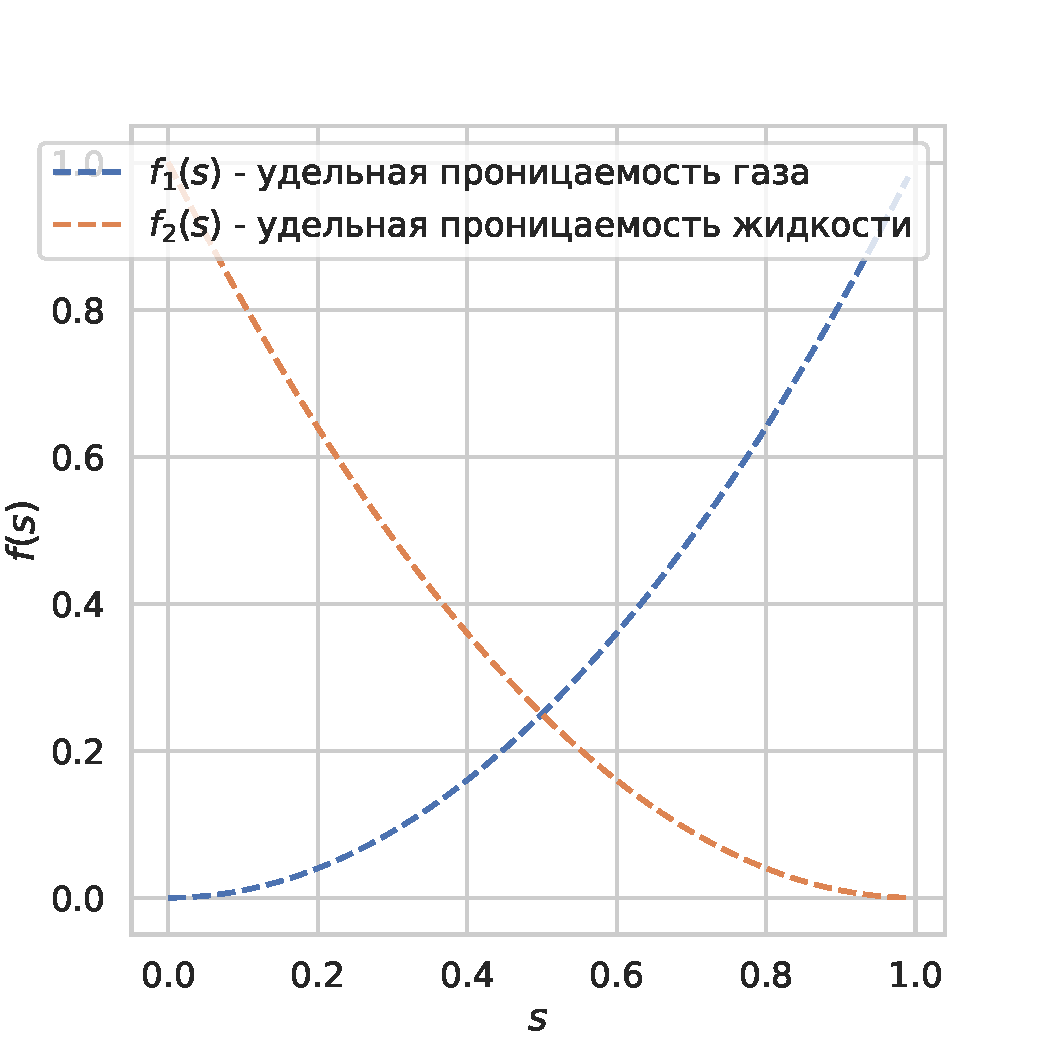
\includegraphics[width=\textwidth]{img/two-phase.pdf}
            \label{fig:}
        \end{figure}
    \end{column}
    \end{columns}
\end{frame}
